\chapter{Domain Diagramm}
Domain Diagramm in kompletter Form:
\begin{figure}[H]
\centering
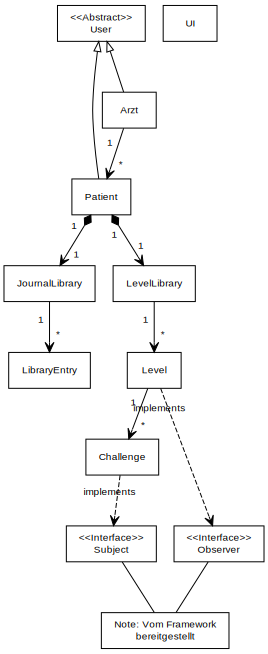
\includegraphics[width=\textwidth,height=.7\textheight,keepaspectratio]{../DomainDiagramms/Full.png}
\caption{Domain Diagramm Full}
\end{figure}

\section{Users}
In diesem Diagramm sehen wir das detaillierte Klassen Diagramm für die User unseres Tools:
\begin{figure}[H]
\centering
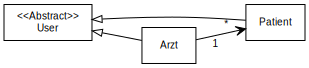
\includegraphics[width=1\textwidth]{../DomainDiagramms/Users.png}
\caption{Domain Diagramm Users}
\end{figure}
Wir haben für die Benuzter eine abstrakte Klasse "User", welche von den Klassen "Patient" und "Arzt" geerbt wird. Die Klasse Arzt hat zusätzlich eine Referenz auf die Patienten Klasse. Das Ziel dabei ist, dass Ärzte die Möglichkeit haben auf die Fortschritte ihrer Patienten zuzugreifen.

\section{Journal}
In diesem Diagramm sehen wir die Details der Journal Klasse:
\begin{figure}[H]
\centering
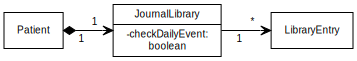
\includegraphics[width=1\textwidth]{../DomainDiagramms/Journal.png}
\caption{Domain Diagramm Journal}
\end{figure}
Das Ziel des Journal ist es, dass Patienten eine Art Tagebuch führen können. Dafür haben wir eine Journal Library Klasse welche die Journal Einträge speichert und zusätzliche Funktionen bereitstellt.
\newpage
\section{Challenges}
Hier sehen wir die Details der Klasse für die Challenge.
\begin{figure}[H]
\centering
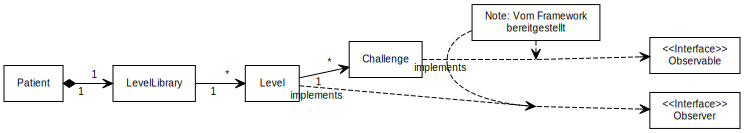
\includegraphics[width=1\textwidth]{../DomainDiagramms/Challange.png}
\caption{Domain Diagramm Challenge}
\end{figure}
Auch für die Levels haben wir eine Level Library welche die einzelnen Levels speichert. Die Level Klasse soll die einzelnen Challenges speichern. Zusätzlich haben wir uns entschieden für die Level und Challenge Klassen ein Observable Pattern zu verwenden. Ziel ist die Umkehrung der Abhängigkeit zwischen Level und Challenge. Die Interfaces "Observer" und "Observable" werden durch das Java Framework bereitgestellt, diese müssen nur noch implementiert werden.

\section{Data Layer Klassen}
\begin{figure}[H]
\centering
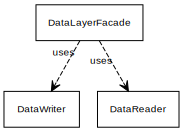
\includegraphics[width=1\textwidth]{../DomainDiagramms/DataLayer.png}
\caption{Domain Diagramm Data Layer Klassen}
\end{figure}
